\newpage

\subsection{Continuous Query Engine - $\mathsf{DP_{ATM}}$}\label{ContinuousQueryEngine}

\textcolor{gray}{To explain:
\begin{itemize}
    \item Encaje/Uso del DP para nuestro engine. Stages, qué hace cada stage (pseudocodigo/algoritmo de cada stage). Canales.
    \item Establecer algoritmos para identificar los patrones asociados a la busqueda de anomalias.
    \item Explicar la idea de que se define como para poder evaluar muchas continuous queries de forma simulatánea (pero que de momento sólo evaluamos una, para nuestro proof of concept)
    \item Detalles más técnicos - Implementación
    \begin{itemize}
        \item Descripción y evaluación del lenguage usado (golang)
        \item Graph-based query language
        \item Tools \& proper system configuration (distintas configuraciones en base al número máximo de tarjetas que contiene cada filtro...)
    \end{itemize}
    \item Windowing?
\end{itemize}
}
\ad{El windowing no lo menciones hasta las conclusiones.}

In this section we define a proper architecture of a continuous query engine for detecting anomalous ATM transactions on a continuous, unbounded, input stream of card-ATM transactions/interactions. We propose an engine that is modeled following the Dynamic Pipeline Paradigm $\mathsf{DPP}$ (see \ref{DPP}), the $\mathsf{DP_{ATM}}$, where, by definition, its architectural framework gets defined as a \DP.\\ 

\fmc{Encaje/Uso del DP para nuestro engine. Volatile subgraphs, cards, filters... Explicar la idea de que se define como para poder evaluar muchas continuous queries de forma simulatánea (pero que de momento sólo evaluamos una, para nuestro proof of concept)}

\fmc{Subgrafos}
The core idea of the \DPATM is to save and construct \emph{volatile} subgraphs of interactions for each of the cards, with the objective to keep track of the ATM transaction/interaction activity of each of the cards of the bank system. The card subgraphs are constructed with the interactions belonging to a certain card. They are defined as \emph{volatile} in the sense that the interactions that compose them are not intended to remain infinitely in the card subgraph, but only for a decided window of time. 
\fmc{Evaluación de muchos tipos de queries de forma simultanea. Un subgrafo por cada tipo de query}
These card subgraphs are the core object on which the detection queries of anomalous PG graph patterns takes place. For each card and for each continuous query pattern, a card subgraph is maintained, allowing the evaluation of many continuous different queries simultaneously. Note that, for each card, a different subgraph for each kind of continuous query is defined due to the possible many distinct time window policies for each particular kind of query.

\fmc{TODO: Poner un dibujo de un subgrafo volátil}

% Descripción general uso DP
To properly characterize the \DP architecture we need to define the configuration and behavior of each of the stages as well as the channels connecting them. The different stages are connected by two communication channels: the \eventch channel carries the interactions of the input data stream and the \alertch channel, which is a direct channel that connects each \emph{Filter} stage with the \sink stage, carries the alerts corresponding to the different possible anomalous transaction patterns detected in a \filter.

\fmc{Duda channels: sólo el de alerts o el de checks. Ahora en la impl tengo checks (incluidos los alerts). Se hizo con la idea de sacar todos los resultados de los checks para ver el continuous delivery of results en los experimentos. Ahora bien, en la impl. final yo diria que solo sacaría las alerts, para tener menos overhead y que el aviso de fraude pudiera llegar antes.}

\ad{Para explicar puedes poner el de checks y que se vea que se van haciendo muchos checks y sólo algunos provocan alerts. Luego puedes explicar que en una "working" version no se pondrías los checks para ser más eficientes y tardar menos en dar los alerts como bien dices.}

Regarding the stages, the \emph{Filter} stage is defined to be the \textit{continuous query evaluator} for a certain subset of bank cards, maintaining the subgraphs for the cards subset that are induced by the interaction edges.

% IDEA GENERAL DP-ATM flow
With this, the \DPATM algorithm overview is as follows: when an interaction $\mathsf{e}$ (with its properties' values) arrives to the \DPATM, the \source stage \Sr registers it into a standard transactional log file. Then, \Sr passes $\mathsf{e}$ to the next stage. If there exists a \filter parameterized with the value of the property \emph{number\_id} of the Card vertex $\mathsf{c}$ that is incident to $\mathsf{e}$, this \filter keeps $\mathsf{e}$ in its state, in particular adding $\mathsf{e}$ to the corresponding card subgraphs. Otherwise, the \filter passes $\mathsf{e}$ to the next stage. In the case of  $\mathsf{e}$ belonging to the \filter, this stage, as the \textit{continuous query evaluator} of the Card $\mathsf{c}$, decides if there is a match with (some of) the continuous query pattern(s) evaluated and emits an alert to the \sink \Sk reporting the finding. Hence, answers are the detected anomalies and they are emitted as they are obtained in filters. When answers/alerts arrive to \Sk, this stage post-processes and output them. In addition, \Sk maintains an answer log file. The fact that an interaction arrives to \G means that there were not previous interactions having the same value of Card property \emph{number\_id} and thus, a new filter parameterized with this new value is spawned. 

\fmc{TODO: Poner imagen de DP con filtros y cada filtro con los subgrafos}

% Descripción más concreta DP...

More detail regarding each of the stages behavior is provided next. An example of the pipeline schema of a \DPATM instance is shown in Figure \ref{img:pipeline-schema}.

\begin{itemize}
    \item \source \Sr: Receives the stream of the card-ATM interactions of the bank. Each interaction $\mathsf{e}$ is represented as an \emph{interaction} relation/edge of the volatile property graph model matching a Card and an ATM \ref{section:volatile-pg}. \Sr registers incoming interaction $\mathsf{e}$ on a transactional log file and passes $\mathsf{e}$ through the \eventch channel to the pipeline.
    \item \filter \F: \emph{Filters} are defined to be the \textit{continuous query evaluators} for a certain subset of the bank system cards. In particular each \F is defined by a subset of root parameters $V_{\mathsf{F}} = \{v_1,\ldots,v_k\}$, representing the Cards being tracked by \F. Therefore, each root represents a Card $\mathsf{c}$ where $v_i$ is the Card property \emph{number\_id} value: $v_i = \mathsf{c}$.\emph{number\_id}. Each \filter is defined to have a maximum capacity in terms of cards being tracked. This maximum capacity is defined by the parameter \emph{maxFilterSize}. This limits the maximum size of the subset $V_{\mathsf{F}}$, so that $|V_{\mathsf{F}}| \leq $ \emph{maxFilterSize}.

    With this, whenever an interaction $\mathsf{e}$ coming from the pipeline reaches \filter \F, it firsts checks whether $\mathsf{e}$ belongs to \filter \F. This is the case when $\mathsf{e}$ is incident to one of the roots of $V_{\mathsf{F}}$, $v_i$, which has the same \emph{number\_id} property value as the Card $\mathsf{c}$ of the interaction $\mathsf{e}$ ($\mathsf{e}$.\emph{number\_id}), that is when $v_i =\mathsf{e}$.\emph{number\_id}. This means that \F is currently tracking the activity of the Card $\mathsf{c}$ to which the interaction $\mathsf{e}$ belongs. 

    \fmc{Se explica cómo se tiene hasta ahora. Pero se debería de explicar una propuesta para el caso en el que se dejara de trackear la actividad de una tarjeta / cómo sería el proceso para poder destruir un filtro/reducir el pipeline.\\
    \textbf{Hasta ahora}: If the filter is not full then we add the not belonging cards to it, until it is full. This is what is done so far, since we are not considering the case to shrink the pipeline. On which some cards activity will be stopped to being tracked. \\
    TODO: Definir una posible propuesta para esto en el caso de que se hiciera... relacionado con lo de la ventana...\\
    - Spawning case is well defined.\\
    - Shrinking case idea: all the cards of the filter have to be "outdated" so that the filter can be eliminated... (not done for the moment, infinite window considered)
    }
    Another possible case on which $\mathsf{e}$ is decided to belong to \filter \F, is when, although the Card $\mathsf{c}$ of $\mathsf{e}$ is not currently being tracked by \F, it is decided to start doing it since \F still has the capacity to track more cards: $|V_{\mathsf{F}}| < $ \emph{maxFilterSize}. Therefore, card $\mathsf{c}$ is introduced as a new root parameter $v_{k+1} = \mathsf{e}$.\emph{number\_id} to $V_{\mathsf{F}}$: $V_{\mathsf{F}} = V_{\mathsf{F}} \cup v_{k+1}$. These two belonging conditions are summarized as:
    
    $$
    \mathsf{e} \in \mathsf{F} \iff 
    \left(\exists v_i \in V_{\mathsf{F}} \text{ such that } v_i = \mathsf{e}.\emph{number\_id} \right) 
    \lor \left(|V_{\mathsf{F}}| < \emph{maxFilterSize}\right).
    $$

    Otherwise ($\nexists v_i \in V_{\mathsf{F}} \text{ such that } v_i = \mathsf{e}.\emph{number\_id} \land |V_{\mathsf{F}}| = $ \emph{maxFilterSize}), \F passes $\mathsf{e}$ to the next stage.

    In the case of $\mathsf{e}$ belonging to \F, \F checks if there is a match with (some of) the continuous query pattern(s) evaluated and emits an alert(s) to the \sink \Sk. For this, $\mathsf{e}$ will be added to the corresponding card $\mathsf{c}$ subgraph(s) with root $v_i =\mathsf{e}$.\emph{number\_id}, and then perform the algorithm to test (each of) the continuous query pattern(s) with their associated card $\mathsf{c}$ subgraph(s). 

    \fmc{Esto justificarlo así?}
    For a card $\mathsf{c}$, we will store one different subgraph for each of the continuous query patterns evaluated. A different subgraph for each of the continuous query patterns is needed since the evaluation politics of each of the patterns may be different. For instance, for a specific pattern we may need to store a full list of interaction edges with some specific properties, whereas for others only the last interaction edge. Or even just some specific properties and not a subgraph of interactions. This will depend on the definition on each of the specific continuous query patterns considered.

    The test of a continuous query pattern is done by means of its associated card \emph{continuous query pattern subgraph} stored by \F and the information retrieved from the stable PG to identify patterns and solve constraints. This is, indeed, the way to evaluate continuous queries.
    
    \item \generator \G: Is the stage in charge of stretching the pipeline by spawning new \filter \F stages when needed. In particular this is the case whenever an interaction $\mathsf{e}$ arrives to \G. At this point this means that there was no \F in the pipeline to which this interaction belonged. That is, whenever no \F was tracking the activity of the Card $\mathsf{c}$ with property value \emph{number\_id} to which this interaction corresponds and all the running \F were full of capacity in terms of the number of maximum cards \emph{maxFilterSize} that they can track. In this case a new \F is spawned, initially tracking the activity of this Card $\mathsf{c}$ with property value \emph{number\_id} and creating new card subgraphs with the interaction $\mathsf{e}$. 
    \item \sink \Sk: It is in charge of receiving all the alerts coming from the \filter stages and to correspondingly act on them as the bank requires. This could be done in terms of communicating the alert to the corresponding cardholders, emitting a message for validating that the operation was done by the owner, freezing the corresponding cards, and so on. This will have to be defined by the corresponding bank as desired. In any case, \Sk maintains an answer log file where all the emitted alerts are registered. Additionally, an event log file is maintained, to register other internal system events.
\end{itemize}


\begin{figure}[H]
    \centering
    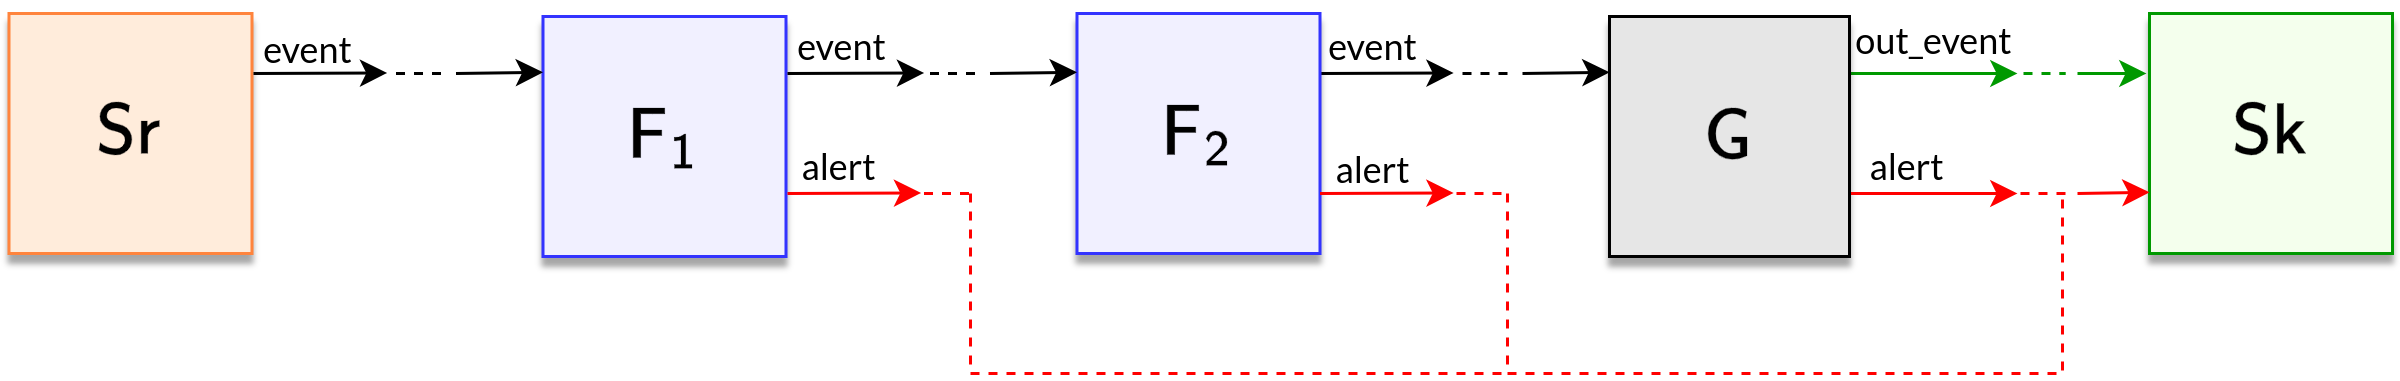
\includegraphics[scale = 0.8]{images/3-Engine/DP-2f.png}
    \caption{Example of the Pipeline Schema of a \DPATM Instance}
    \label{img:pipeline-schema}
\end{figure}


\fmc{Windowing?}
When the time interval window is over, the $\mathsf{DP_{ATM}}$ is, in some sense, reset according to the given window policy. Note that the window policy must take into account stored data that might be valid in between two windows and handle the transition properly.

\fmc{Detalles técnicos - Implementación}
\subsection*{$\mathsf{DP_{ATM}}$ - Implementation}\label{ContinuousQueryEngine-Implementation}

% Lenguaje de programación. Base de datos. Conexión a base de datos.
% - Go: Detalles versión. Por qué lo usamos
% - Neo4j: Detalles versión. Por qué lo usamos
The implementation of the proof of concept can be found in Github\footnote{\url{https://github.com/FCanfran/ATM-DP}}. It was developed using the version \texttt{1.20} of the \texttt{Golang} language. 
% Ventajas: hilos verdes - concurrencia, comunicación entre stages con canales de fácil manejo, fácil conexión con Neo4j mediante el driver
One of the main reasons why we decided to use this language is its inherent capacity to support concurrent programming \cite{Go-cbtnuggets_concurrency, Go-medium_concurrency, Go-reliasoftware_concurrency}, which is the computing technique that we need to implement the \DP schema for our \DPATM engine. In \texttt{Go}, concurrency is achieved primarly through \texttt{goroutines} and \texttt{channels}. \texttt{Goroutines} are lightweight, independent concurrent green threads, which are managed by the \texttt{Go} runtime scheduler, and enable concurrent execution of functions, in our case stages. The communication between \texttt{goroutines} is accomplished via different channels. This provides a safe and efficient method to pass complex data between the different \texttt{goroutines}. 
Unlike traditional threads, \texttt{goroutines} have a small memory footprint and can be created in large numbers with minimal overhead. The \texttt{Go} runtime includes an efficient scheduler that multiplexes \texttt{goroutines} onto CPU cores, reducing context switching overhead and optimizing resource use. However note that, \texttt{goroutines} are not inherently parallel. By default, \texttt{Go} uses only one operating system thread, regardless of the number of \texttt{goroutines}. We need to set up the \texttt{GOMAXPROCS} \footnote{\url{https://pkg.go.dev/runtime\#GOMAXPROCS}} environment variable to the number of logical processors, to achieve that the \texttt{Go} runtime scheduler multiplexes the \texttt{goroutines} onto all the possible logical processors specified.\\

Another advantage that made the election of \texttt{Go} quite suitable was its easy form to interact with \texttt{Neo4j}. \texttt{Go} provides the \texttt{Neo4j Go driver}\footnote{\url{https://neo4j.com/docs/go-manual/current/}} to easily interact with a Neo4j instance through a \texttt{Go} application. More details regarding the connection are later explained. 

\subsubsection*{Neo4j Connection}\label{Neo4j-connection}
% Detalle de la conexión con Neo4j
Our \DPATM system needs a way to interact with the stable bank database PG instance in order to retrieve additional information related with the cardholders or ATMs for the evaluation of the continuous queries. The connection to the Neo4j graph database instance that represents the stable bank PG database is implemented using the version \texttt{v5.24.0} of the \texttt{Neo4j Go driver}\footnote{\url{https://pkg.go.dev/github.com/neo4j/neo4j-go-driver/v5@v5.24.0/neo4j}}. Next we give an overview of some important details on the usage of this driver in order to connect and query the Neo4j instance. More detail on the methods we used can be found in the official driver module websites \cite{neo4j-go-neo4j_go_driver, neo4j-go-neo4j_go_manual}.\\


In our implementation of the \DPATM system in \texttt{Go} we developed the \texttt{Go} module \texttt{internal/connection} to deal with the connection management with the Neo4j stable bank graph database instance.
On it we provide all the needed functions to connect to the database, create connection sessions, and to query it. 

% Initial connection method - .env... driverwithcontext
% Sessions for each of the filters
% Query method to run cypher queries...

\begin{itemize}
    \item \textbf{Initial connection setup}: The \DPATM system initially sets up the connection through the creation of a \texttt{DriverWithContext} object.\\
    In the \texttt{internal/connection} module \texttt{SafeConnect()} is the function that we implement to construct the \texttt{DriverWithContext} object and verifies that a working connection can be established through the \texttt{.VerifyConnectivity()} method.
    The \texttt{DriverWithContext} object holds the details required to establish connections with a Neo4j database, allowing connections and creation of sessions. It is a sharable object among threads. To provide the required details we used the module package \texttt{godotenv}\footnote{\url{https://pkg.go.dev/github.com/joho/godotenv}} to obtain the \textit{URI} and the credentials from a \texttt{.env} file, where the related environment variables are specified. For the connection with our Neo4j instance we use the \texttt{Bolt}\footnote{\url{https://neo4j.com/docs/bolt/current/bolt/}} application protocol, which is the protocol used for interaction between Neo4j instances and drivers. It listens on port 7687 by default. 
    To illustrate, we show an example of a \texttt{.env} file, from which the connection credentials will be gathered by our application. On it the connection details of a toy local Neo4j instance are shared:

    \begin{center}
    \lstset{style=cypherStyle}
    \begin{lstlisting}[caption={Example of a \texttt{.env} file, from which from which the connection credentials will be gathered by our \DPATM application.}]
        NEO4J_URI="bolt://localhost:7687"
        NEO4J_USERNAME="neo4j"
        NEO4J_PASSWORD="xxxxx"
    \end{lstlisting}
    \end{center}

    \item \textbf{Connection sessions}: \texttt{Sessions} act as concrete query channels between the driver(\texttt{DriverWithContext} object) and the server. We need them in order to be able to run \texttt{Cypher} queries from each of the working \filter stages. Each \filter stage creates a different \texttt{session} to interact with the Neo4j database.
    
    In the \texttt{internal/connection} module, the functions \texttt{CreateSession(...)} and \texttt{CloseSession(...)} are the functions for the creation and closing of a \texttt{session}.
    They are created from the \texttt{DriverWithContext} object. 

    \item \textbf{Running queries}: We provide the methods \texttt{ReadQuery(...)} and \texttt{WriteQuery(...)}, which create a \textit{managed transaction} to retrieve data from the database or alter it, respectively, through a \texttt{Cypher} statement. 
    Internally they call the \texttt{ExecuteRead(...)} and the \texttt{ExecuteWrite(...)} functions of the \texttt{Neo4j Go Driver}, which execute the given unit of work in a read/write transaction, via the provided session.

    In the \DPATM we make use of the \texttt{ReadQuery(...)} function from each of the \filter stages, using its own \texttt{session}, to query the database using \texttt{Cypher} statements.
\end{itemize}

\fmc{DUDA: Pongo una referencia a esto?}
\textcolor{gray}{Neo4j limits the number of parallel transactions to 1000 by default. However, so far no reference regarding the limit on the number of parallel sessions has been found. In any case, it is important to remark that many multiple parallel sessions may cause overhead to the database. This can be the case for the architectural design we are proposing, where we have a session per each \filter stage.}

% Comunicación. Canales, tipos más concretos. Eventos, tipos de eventos concretos. Start and End Edges.
\subsubsection*{Communication}

The communication of the different stages is carried via different \texttt{Go} channels. In general, although otherwise specified all the channels that we use are buffered channels of size 5000. All the channels are described next:

\begin{itemize}
    \item \eventch: \texttt{event} channel. Its main purpose is to carry the interaction edges across the \DP stages, from \Sr to \G, passing by all the \F's. The \texttt{event} data type consists on a \texttt{EventType} label and in a \texttt{Edge} object. The \texttt{EventType} label indicates the type of event that can be either: \texttt{EdgeStart} representing an opening of an interaction, \texttt{EdgeEnd} representing an interaction closing, \texttt{EOF}, representing the \textit{End Of File} event so that the \DP can become to an end, finalizing all the stages, and the \texttt{LOG} event for internal log messages of the system.
    \begin{center}
    \lstset{style=golangStyle}
    \begin{lstlisting}[caption={\texttt{Event} Data Type}]
                type Event struct {
            	   Type      EventType
            	   E         Edge
                }
    \end{lstlisting}
    \end{center}

    \texttt{Edge} is the data type that we defined for the interaction edges. This object will be relevant in the case of the \texttt{EdgeStart} and \texttt{EdgeEnd} events, since in this case the \texttt{Edge} object will be containing the information of the opening and closing interaction, respectively, as defined in the volatile property graph data model definition (see \ref{section:volatile-pg}).
    
    % Tipo de dato interaction edge Edge
    \begin{center}
    \lstset{style=golangStyle}
    \begin{lstlisting}[caption={Data Type for the interaction edges in Go}]
    type Edge struct {
    Number_id string   // Card id
    ATM_id   string    // ATM id
    Tx_id    int32     // id
    Tx_type  TxType    // type (withdrawal/deposit/inquiry/transfer)
    Tx_start time.Time // start datetime(DD/MM/YYYY HH:MM:SS)
    Tx_end   time.Time // end datetime(DD/MM/YYYY HH:MM:SS)
    Tx_amount float32  // amount
    }
    \end{lstlisting}
    \end{center}

    where \texttt{TxType} is a custom type made for the different interaction types: 
    \texttt{withdrawal}, \texttt{withdrawal}, \texttt{withdrawal} and  \texttt{withdrawal}. 

    \begin{center}
    \lstset{style=golangStyle}
    \begin{lstlisting}[caption={\texttt{TxType} Data Type, for the different interaction types}]
            type TxType uint8
            const (
            	Withdrawal TxType = 0
            	Deposit           = 1
            	Inquiry           = 2
            	Transfer          = 3
            	Other             = 4
            )
    \end{lstlisting}
    \end{center}
    
    \item \alertch: \texttt{alert} channel. It carries the alerts corresponding to the different possible anomalous transaction patterns detected in a \filter. It is a channel directly connecting each of the \emph{Filters} with the Sink stage. This means that when an alert is emitted it does not have to travel through all the remaining \F stages of the \DP nor the \G stage, allowing a faster communication of the alert to the \Sk stage, in charge of processing the alerts. The \texttt{alert} data type consists on a \texttt{Label} to indicate the type of fraud pattern to which it corresponds, an \texttt{Info} string to indicate additional information related with the alert, and finally \texttt{Subgraph}, the subgraph data structure that triggered the alert. Note that this subgraph does not need to be the full subgraph of the card that triggered the alert, it can be just the part of it involved in the alert. For instance, in the case of the fraud pattern I, these subgraph is composed of the two interaction edges that caused the trigger of this kind of fraud pattern alert.
    \begin{center}
    \lstset{style=golangStyle}
    \begin{lstlisting}[caption={\texttt{Alert} Data Type}]
    type Alert struct {
    	Label    string        
    	Info     string        
    	Subgraph Graph         
    }
    \end{lstlisting}
    \end{center}
    \item $\mathsf{out\_event}$: direct dedicated \texttt{event} channel between the \G and \Sk. 
    \item $\mathsf{internal\_edge}$: Internal \texttt{event} channel between a \F stage and its related \FW substage. It only pass interaction \texttt{Edge} events (\texttt{EdgeStart} and \texttt{EdgeEnd}), that have been determined to belong to the \filter, so that the related \FW of \F can do the corresponding processing with it.
  \end{itemize}

% Detalle de las estructuras y los métodos usados en cada una de las stages.
\subsubsection*{Stages}
In what follows we give specific implementation details of each of the stages of the \DP paradigm used for the \DPATM. Each stage takes the form of a \texttt{goroutine} of the \texttt{Go} language.

% - Source: como se hace la lectura. Como se empezó haciendo inicialmente y cómo se decidió hacer finalmente (lectura por chunks) - hacer referencia a apartado de experimentos donde mostrar el experimento hecho para enseñar que era mejor.
\paragraph*{Source\\ }

% Explicar función

\source stage is designed to be the connection point of the \DPATM with the bank ATM network to receive the interactions produced on these ATMs, which compose the input interaction stream.\\

\fmc{DUDA: Aqui esto no se como ponerlo...
- Decir algo de kafka message queue (como en seraph)?
}
% Forma real de cómo sería el source: recibiendo flujo de transacciones en real time
% Cómo lo hacemos nosotros - lectura de fichero - y variantes dependiendo del tipo de experimento que realizamos
In a real-case scenario, these interaction events could be sent by the ATMs of the bank network and be received by a message queue on our \DPATM system. For our proof of concept, where we generated our own synthetic stream of transactions in a \texttt{csv} file,
the interactions are read from these files, parsed into \texttt{Edge} data types and provided to the pipeline in different ways depending on the kind of simulation we perform. As it will be shown in the Experiments section, we implemented two different cases of simulations. The real-case scenario and the high loaded test scenario. In the first case, the interactions, although read by a file of artificial simulated interactions, are provided to the pipeline data stream in such a way that they simulate their actual arrival time to the system, with the corresponding time separation between them. In the second case, the interactions are provided just one after the other as fast as possible as they are read.\\

% Cómo se leen, parsing al tipo de dato Edge...
In any case, we want the reading of the input file to be the fastest possible, so to minimize the potential bottleneck derived from the operation of reading a file, we utilized a buffered reader of the \texttt{bufio} package, which reads chunks of data into memory, providing buffered access to the file. This buffered reader was provided to a \texttt{csv} reader of the \texttt{encoding/csv} package to read the buffered stream as \texttt{csv} records.

    \begin{center}
    \lstset{style=golangStyle}
    \begin{lstlisting}[caption={\texttt{csv-bufio} reader}]
        reader := csv.NewReader(bufio.NewReader(file))
    \end{lstlisting}
    \end{center}
    
% Lectura por chunks
% chunk size = 100
% read with the help of a worker to keep reading in the background, to accelerate the reading -> explain the reason of why this
Another optimization that was done in order to be able to minimize this bottleneck on the reading of the interactions from the \texttt{csv} file, was reading by chunks the \texttt{csv} records/rows. In particular, this was done by having a \textit{worker} subprocess, implemented as an anonymous \texttt{goroutine} inside \Sr, whose task was to continuously read records from the file using the \texttt{csv-bufio} reader accumulating them in a chunk of rows that were provided through a channel to \Sr whenever they reached the defined \emph{chunkSize}. These records were read directly as \texttt{string} data types. On its side, whenever \Sr receives a chunk of rows, it takes each of the rows on it, parses it to the \texttt{Edge} data type and sends it through the pipeline to the next stage.\\

The \emph{chunkSize} was selected to be of $10^2$ rows. In \ref{exps-input-reading} we provide an experimental analysis that proves and justifies the benefits of this buffered and chunked file reading. On it the \texttt{encoding/csv} package performance is compared to other variants using the \texttt{apache/arrow} package with different combinations of \emph{chunkSize}. We also analyze the benefits of introducing the \textit{worker} subprocess to perform the chunked reading.

\fmc{Explicar más en detalle como va lo de la lectura por chunks con el worker?}







% - Filter: forma inicial - sin filter worker y 1 card per filter - y mejoras posteriores con filter-worker y varias cards por filtro con un hash map para indexar... Poner esquema/algoritmo final del filtro (con referencia al algoritmo de FP definido en el query model).
\paragraph*{Filter\\}

Regarding the \filter stage, there are four main aspects worthy to describe on its implementation: the card subgraph data structure implementation, the \emph{decoupled event handling} implementation, the \filter multiple cards support and the continuous query evaluation.
\begin{itemize}
    \item \textbf{Card Subgraph Data Structure}\\
    It contains the interaction edges related with the continuous query fraud pattern evaluation of a specific card.
    The card subgraph data structure is selected based on the fraud patterns considered so far. Although for the implementation of the detection of the fraud pattern I (see \ref{section:queryModel}) we only need to store the last/most recent interaction for each card, we propose a \texttt{Go} \texttt{list} of \texttt{Edge} (interaction edges) objects as a more general data structure to store incoming interactions ordered by timestamp. This decision responds to what we see it is a more general data structure ready for its usage when implementing the detection of other kinds of fraud patterns.\\ 

    \begin{center}
    \lstset{style=golangStyle}
    \begin{lstlisting}[caption={Card Subgraph Data Structure in Go}]
    type Graph struct {
    	edges *list.List 
    }
    \end{lstlisting}
    \end{center}

    A card subgraph is constructed based on the belonging interaction edges that arrive in the form of incoming \texttt{EdgeStart} and \texttt{EdgeEnd} events. \texttt{EdgeStart} event  produces the creation of a new \texttt{Edge} on the data structure, whereas a \texttt{EdgeEnd} event completeS the values of the properties of the corresponding \texttt{Edge} on the data structure, that was previously created by the \texttt{EdgeStart} event corresponding to that same ATM-Card interaction.

    \fmc{TODO: Poner dibujito de subgrafos dentro del filtro?}

    \item \textbf{Decoupled Event Handling}\\
    % Filter worker
    We implement a \emph{Decoupled Event Handling}, as in the \DP implemented on \cite{DP-Benedi_Garcia_2024}. As the authors mention in this work, there exists a potential inefficiency in the way that the \filter \F stage is defined to work: if an event belongs to the filter then it does the processing related to it. Until \F does not complete this processing the events that arrive to it are not being able to be handled, even if the event does not belong to \F. We have the same scenario for the \DP of the \DPATM, where the events that can belong to \F are the interaction edge $\mathsf{e}$ events.

    To avoid this bottleneck on the flow of interaction edge $\mathsf{e}$ events, the \filterworker \FW is introduced as a substage of the \filter \F stage. \F and its associated \FW will be running in different \texttt{goroutines}. The idea is that \F acts as a dedicated \textit{mailbox}, reading the events coming from the \texttt{event} channel and \emph{filtering} them, that is, deciding whether an incoming interaction edge $\mathsf{e}$ belongs to \F or not. In the case $\mathsf{e}$ belongs to \F, \F forwards $\mathsf{e}$ to the \FW, otherwise it continues passing $\mathsf{e}$ through the pipeline. \FW is dedicated to do the corresponding processing with the interaction edges belonging to the stage that are forwarded by \F.\\

    This decoupling allows to do the processing of belonging interaction edges while not blocking the pipeline event flow, since at the same time it does the \emph{filtering} of events.\\

    In our \texttt{Go} implementation, we decided to implement \FW as an internal anonymous \texttt{goroutine} of the \F \texttt{goroutine}, instead of an external (named) \texttt{goroutine}. 

    To communicate the interaction edges between \F and \FW we use an internal channel \internaledgech. Another possible option considered was a shared buffer of interaction edges. In this last case a mutex would have been needed, since \F and \FW can possible write and read, respectively, into this buffer at the same time. The \textit{mutex} is needed to avoid race conditions in the sharing of the buffer. 
    However, channels are a much more simple alternative to lead with this communication, as they are specifically designed for synchronization and passing the ownership of data, which is the case we are dealing with. Some references on the preference usage of channels over mutex \cite{Go-channels-mutex-gowiki_mutex_channel, Go-channels-mutex-stackoverflow_mutex_channel}.

    The decision to implement \FW as an internal anonymous \texttt{goroutine} also provided a way to simplify the code, since \FW can access the variables of the scope of \F (no need to pass them as parameters). This is particularly useful in the case of the \alertch channel, to which \FW is able to write directly. Same in the case of the \internaledgech channel.

    \begin{figure}[H]
      \centering
      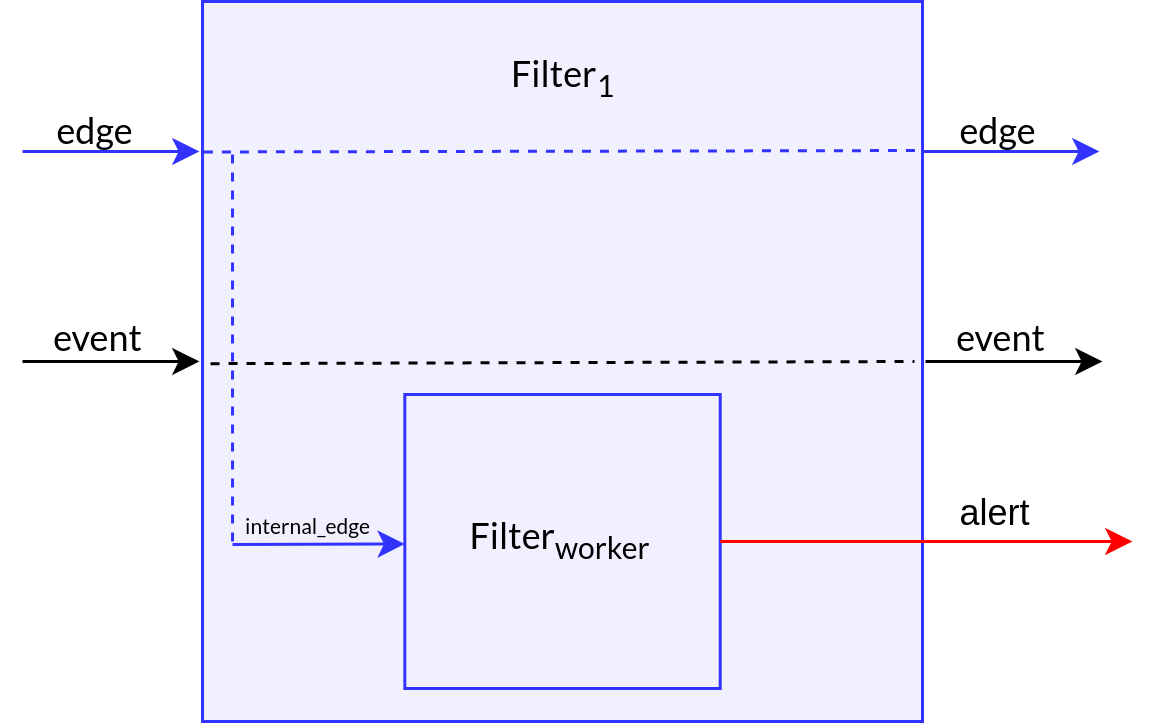
\includegraphics[scale = 1.2]{images/3-Engine/filter-worker.png}
      \caption{Filter Worker detail}
      \label{img:pipeline-schema}
    \end{figure}

    \item \textbf{Multiple Cards Support}\\
    In an initial first toy implementation, we were tracking the activity of only one card per \filter, meaning that for each bank card we were dedicating a \texttt{goroutine} on the form of a \filter stage. This was done as a way to get started, it fast became obvious that this is was an unnecessary waste of computational resources. On a real case scenario, where the number of ATM-card interactions a bank card in a day is not expected to be higher than one on average \fmc{TODO: Poner una referencia formal}, it became clear the need of allowing to share each \filter stage for multiple bank cards.\\

    Formally, as described on \ref{ContinuousQueryEngine}, each \filter \F was implemented to be able to hold a certain subset of root parameters $V_{\mathsf{F}} = \{v_1,\ldots,v_k\}$, representing the Cards being tracked by \F.\\

    In \texttt{Go} to achieve the support of multiple cards per \filter we decided to use hash tables. Go provides a built-in \texttt{map} type that implements a hash table\footnote{\url{https://go.dev/blog/maps}}. We used two different maps, using the card id of the interaction edge $\mathsf{e}$.\emph{number\_id} as the key of both maps.

    \begin{itemize}
        \item \texttt{cardList} \texttt{map}: It is used by \F to determine whether an interaction edge $\mathsf{e}$ belongs to \F, $\mathsf{e} \in$ \F. Only accessed by \F.
        \item \texttt{cardSubgraph} \texttt{map}: To index the interaction edge $\mathsf{e}$ to the corresponding card subgraph.
        Only accessed by \FW. Note that, for our proof of concept, as we are considering only one fraud pattern, we only need one \texttt{cardSubgraph} \texttt{map} data structure. However, note that more will be needed if we consider more fraud patterns with different card subgraphs.
    \end{itemize}

    \begin{center}
    \lstset{style=golangStyle}
    \begin{lstlisting}[caption={Hash Tables \texttt{map} Data Structures on a \emph{Filter} \F stage}]
    var cardList map[string]bool = make(map[string]bool)
    var cardSubgraph map[string]*cmn.Graph = make(map[string]*cmn.Graph)
    \end{lstlisting}
    \end{center}

    % Reason why two maps and not only one
    One could think of using one single \texttt{map} data structure to do the check $\mathsf{e} \in$ \F and at the same time index $\mathsf{e}$ to the corresponding card subgraph, if it is the case. However, the reason why we need two \texttt{maps} and not only one is to respect the architecture of the decoupled event handling. On it, we have two \texttt{goroutines} \F and \FW (as an anonymous internal \texttt{goroutine} of \F) dedicated to check $\mathsf{e} \in$ \F and to do the processing of $\mathsf{e}$, respectively. Having only one \texttt{map} data structure, would mean that both \F and \FW would be doing simultaneous read/write operations on the \texttt{map}, which is unsafe as is not defined what happens (possible race conditions) in \texttt{Go} in this situation. The runtime also warned us to avoid this by alerting us with a fatal error message if we try to share this data structure without any kind of synchronization tool: \textit{\textcolor{red}{Issue: "fatal error: concurrent map read and map write"}}. Therefore a \textit{mutex} or a concurrent map implementation like a \texttt{syncmap} would be needed to control the concurrent access to this shared data structure. For simplicity we decided to avoid sharing the data structure and dedicating one \texttt{map} for each of the \F and \FW stages.

    \item \textbf{Continuous query evaluation}\\
    % Explain the checkFraudI function
    % Fraud pattern 1: obtainTmin -> how this is achieved by retrieving the info from the Neo4j gdb...
    % Fraud patter 0 - tx overlapping -> consider it part of the same?
    As already mentioned, the continuous query evaluation of the different fraud patterns for the cards is accomplished in the \filter stage. For a card $\mathsf{c}$ this is achieved with the evaluation of the algorithms that characterize each of the defined fraud patterns. These algorithms are evaluated over the corresponding card subgraphs and the information retrieved from the stable PG bank database, identifying if there is a subgraph that matches the given patterns and satisfies its constraints.\\
    
    So far, we implemented the fraud pattern I, related with the characterization of a card cloning scenario, as defined in the algorithmic description \ref{alg:check-fraud-def}. 
    In \ref{alg:check-fraud-impl} we provide a more detailed description of the implementation of this algorithm. Whenever a \texttt{EdgeStart} event arrives to \FW through the \internaledgech channel the checking algorithm \texttt{checkFraud} is performed. \texttt{checkFraud} is executed over a non-empty card subgraph $\mathsf{S_c}$ and the interaction \texttt{Edge} $\mathsf{e_{new}}$ of the \texttt{EdgeStart} event. It is checked that there exists a sufficient time distance between $\mathsf{e_{new}}$ and $\mathsf{e_{last}}$; the previous added edge to $\mathsf{Sc}$ before $\mathsf{e_{new}}$.\\
    
    To do it, we need to obtain the minimum needed time \texttt{t\_min} to traverse the distance between the ATMs of the $\mathsf{e_{new}}$ and $\mathsf{e_{last}}$ interactions: $\mathsf{ATM_{last}}$ and $\mathsf{ATM_{new}}$, corresponding to the ATMs with identifiers $\mathsf{e_{last}}.\texttt{ATM\_id}$ and $\mathsf{e_{new}}.\texttt{ATM\_id}$, respectively. \texttt{t\_min} is obtained through the function call $\text{obtainTmin}(\mathsf{e_{last}}, \mathsf{e_{new}})$ on line \ref{line:obtainTmin}. This function obtains the location coordinates of the two ATMs through two \texttt{Cypher} query to the Neo4j stable bank database, using the \texttt{ATM\_id} identifiers (see code listing \ref{lst:cypherQueryCoords}). This is needed since, by definition interaction edges do not contain this information, and therefore the stable bank database needs to be queried to retrieve it, so to be able to do the check of this graph pattern. This query is executed using the function \texttt{ReadQuery} from the \texttt{internal/connection} module of our \DPATM implementation.

    \begin{algorithm}[H]
      \small
      \begin{algorithmic}[1]
      \REQUIRE $\mathsf{S_c}$ is a non-empty subgraph of interaction edges of card $\mathsf{c}$, $\mathsf{e_{new}}$ is the \texttt{Edge} related with the new incoming opening interaction \texttt{EdgeStart} of card $\mathsf{c}$
      \STATE $\mathsf{e_{last}} \gets S_c[|S_c| - 1]$ \COMMENT{Retrieve the last edge from the subgraph $\mathsf{S_c}$}
      \IF{$\mathsf{e_{last}}.\texttt{Tx\_end}$ is empty}
          \STATE \texttt{LOG: Warning: A tx ($\mathsf{e_{new}}$) starts before the previous ($\mathsf{e_{last}}$) ends!} 
          \RETURN
      \ENDIF
      \IF{$\mathsf{e_{last}}.\texttt{ATM\_id} \neq \mathsf{e_{new}}.\texttt{ATM\_id}$}
          \STATE $\texttt{t\_min} \gets \text{obtainTmin}(\mathsf{e_{last}}, \mathsf{e_{new}})$\label{line:obtainTmin}
          \STATE $\texttt{t\_diff} \gets \mathsf{e_{new}}.\texttt{Tx\_start} - \mathsf{e_{last}}.\texttt{Tx\_end}$
          \IF{$\texttt{t\_diff} < \texttt{t\_min}$}   
            \STATE $\text{emitAlert}(\mathsf{e_{last}}, \mathsf{e_{new}})$\label{line:emitAlert}
          \ENDIF
      \ENDIF
      \end{algorithmic}
      \caption{\texttt{checkFraud}($\mathsf{S_c, e_{new}}$)}
      \label{alg:check-fraud-impl}
    \end{algorithm}

    
    \begin{center}
    \lstset{style=cypherStyle}
    \begin{lstlisting}[caption={Code of the constructed \texttt{Cypher} query in \texttt{Go} to obtain the location coordinates of an ATM with its id on the Neo4j graph database}, label={lst:cypherQueryCoords}]
    getATMLocationQuery := 
    MATCH (a:ATM) WHERE a.ATM_id = $ATM_id RETURN 
    a.loc_latitude AS loc_latitude, 
    a.loc_longitude AS loc_longitude
    \end{lstlisting}
    \end{center}

    Once the location coordinates of both ATMs are obtained from the query:
    \begin{itemize}
        \item  $\mathsf{coords_{last}} = (\mathsf{ATM_{last}}.\texttt{loc\_latitude}, \mathsf{ATM_{last}}.\texttt{loc\_logitude})$ 
        \item  $\mathsf{coords_{new}} = (\mathsf{ATM_{new}}.\texttt{loc\_latitude}, \mathsf{ATM_{new}}.\texttt{loc\_logitude})$
    \end{itemize}
    
    then \texttt{t\_min} is calculated as: $\texttt{t\_min} = \texttt{distance}(\mathsf{coords_{last}}, \mathsf{coords_{new}})/\ \texttt{maxSpeed}$.\\
    $\texttt{distance}(\mathsf{coords_{last}}, \mathsf{coords_{new}})$ is the great-circle distance or orthodromic distance between the two coordinate points. It is calculated using the \texttt{Go} haversine package\footnote{\url{https://github.com/umahmood/haversine}}.
    
    \texttt{maxSpeed} is a parametrizable constant indicating the maximum speed at which it is assumed that the distance between any two geographical points can be traveled. So far we defined it to be \texttt{maxSpeed} = 500 km/h. This parameter will have to be defined by the bank system. Of course, a more refined version could calculate this minimum time considering more variables, so to provide a more precise calculation.

    If the required conditions hold, then an \texttt{Alert} is emitted through the \alertch channel to the \sink stage. This is summarized on the function $\text{emitAlert}(\mathsf{e_{last}}, \mathsf{e_{new}})$ on line \ref{line:emitAlert}. The \texttt{Alert} will contain the subgraph built with the two interaction edges causing the alert: $\mathsf{e_{new}}$ and $\mathsf{e_{last}}$ on the \texttt{Subgraph} field, as well as the indication on the type of fraud on its \texttt{Label} field as the type "1" and some optional additional information related with the anomaly on \texttt{Info}. A possible implementation of this function is shown in \texttt{Go} in the \ref{lst:emitAlertImpl} code listing. Note that $\mathsf{out\_alert}$ refers to the output \alertch channel that connects the \filter stage with the \sink stage ( \texttt{chan<- cmn.Alert}).

    \begin{center}
    \lstset{style=golangStyle}
    \begin{lstlisting}[caption={Possible implementation of $\text{emitAlert}(\mathsf{e_{last}}, \mathsf{e_{new}})$}, label={lst:emitAlertImpl}]
            var fraudAlert Alert 
            subgraph := NewGraph()
            subgraph.AddEdge(last_e)
            subgraph.AddEdge(new_e)
            fraudAlert.Label = "1"
            fraudAlert.Info = "fraud pattern"
            fraudAlert.Subgraph = *subgraph
            ...
            out_alert <- fraudAlert
    \end{lstlisting}
    \end{center}
\end{itemize}

With all these ingredients a final \texttt{Go} implementation of the \filter is provided on the code listing \ref{lst:filterImplementation}.

\newpage
\begin{center}
\lstset{style=golangStyle}
\begin{lstlisting}[caption={A \filter stage \texttt{Go} implementation}, label={lst:filterImplementation}]
func filter(event cmn.Event, in_event <-chan cmn.Event, out_event chan<- cmn.Event, out_alert chan<- cmn.Alert) {

var edge cmn.Edge = event.E
var cardList map[string]bool = make(map[string]bool)
var cardSubgraph map[string]*cmn.Graph = make(map[string]*cmn.Graph)
cardList[edge.Number_id] = true
internal_edge := make(chan cmn.Event, cmn.ChannelSize)
// termination synchronization channel F-FW
endchan := make(chan struct{}) 

context := context.Background() 
session := connection.CreateSession(context)
defer connection.CloseSession(context, session)

// FW 
go func() {
 // auxiliary subgraph variable
 var subgraph *cmn.Graph 
 cardSubgraph[edge.Number_id] = cmn.NewGraph()
 subgraph, _ := cardSubgraph[edge.Number_id]
 subgraph.AddEdge(edge)
Worker_Loop:
 for {
    event_worker, _ := <-internal_edge
    switch event_worker.Type {
      case cmn.EOF:
      // finish the worker
      endchan <- struct{}{}
      break Worker_Loop
    case cmn.EdgeStart:
      subgraph, ok = cardSubgraph[event_worker.E.Number_id]
      if !ok {
        // first edge related to the card on subgraph
        cardSubgraph[event_worker.E.Number_id] = cmn.NewGraph()
        subgraph, _ = cardSubgraph[event_worker.E.Number_id]
        subgraph.AddEdge(event_worker.E)
      } else {
        // already an edge of the card
        isFraud, alert := subgraph.CheckFraud(context, session, event_worker.E)
        if isFraud {
          alert.LastEventTimestamp = event_worker.Timestamp
          out_alert <- alert
        }
        // set as new head of the subgraph (only save the last edge)
        subgraph.NewHead(event_worker.E)
      }
    case cmn.EdgeEnd:
      subgraph, ok = cardSubgraph[event_worker.E.Number_id]
        if !ok {
          cardSubgraph[event_worker.E.Number_id] = cmn.NewGraph()
          subgraph, _ = cardSubgraph[event_worker.E.Number_id]
          subgraph.AddEdge(event_worker.E)
        } else {
          subgraph.CompleteEdge(event_worker.E)
        }
    }
    }
}()

// Filter
Filter_Loop:
 for {
    event, _ := <-in_event
    switch event.Type {
    case cmn.EOF:
        internal_edge <- event
        <-endchan
        out_event <- event 
        break Filter_Loop
    case cmn.EdgeStart, cmn.EdgeEnd:
        if cardList[event.E.Number_id] {
            internal_edge <- event
        } else if len(cardList) < cmn.MaxFilterSize {
            cardList[event.E.Number_id] = true
            internal_edge <- event
        } else {
            out_event <- event
        }
    }
}
close(internal_edge)
close(out_event)
}
\end{lstlisting}
\end{center}

% - Generator: Descripción. Código concreto?
\paragraph*{Generator\\}

The \generator \G main functionality is spawning a new \filter \F stage whenever it receives an interaction \texttt{Edge} event. This event is provided as a parameter to the new spawned \F so that it can be then processed there.

Whenever the new \F is spawned, the pipeline is reconnected accordingly: \F takes as \eventch input channel the original \eventch input channel of \G, and \G generates a new \eventch input channel which is set up as the output \eventch channel for \F and as the new input \eventch channel for \G. The \alertch is also provided to \F so that it can utilize as an output channel to send alerts to the \sink stage.

\fmc{Poner extracto código para enseñar mejor?}

% - Sink...
\paragraph*{Sink\\}

The \sink \Sk stage is in charge of reading from the \eventch and \alertch. Its main functionality is to receive the \texttt{alerts} coming from the \alertch and post-processing them accordingly to the bank requirements. In our case, we just write them into an output file to record them. In addition we also maintain a log event output file with the received events received from the \eventch channel.

\fmc{Actualizar los dibujos correspondientes. Poner estos y otros similares a los de la presentación del AMW2024 pero actualizados a este formato.}
\begin{figure}[H]
  \centering
  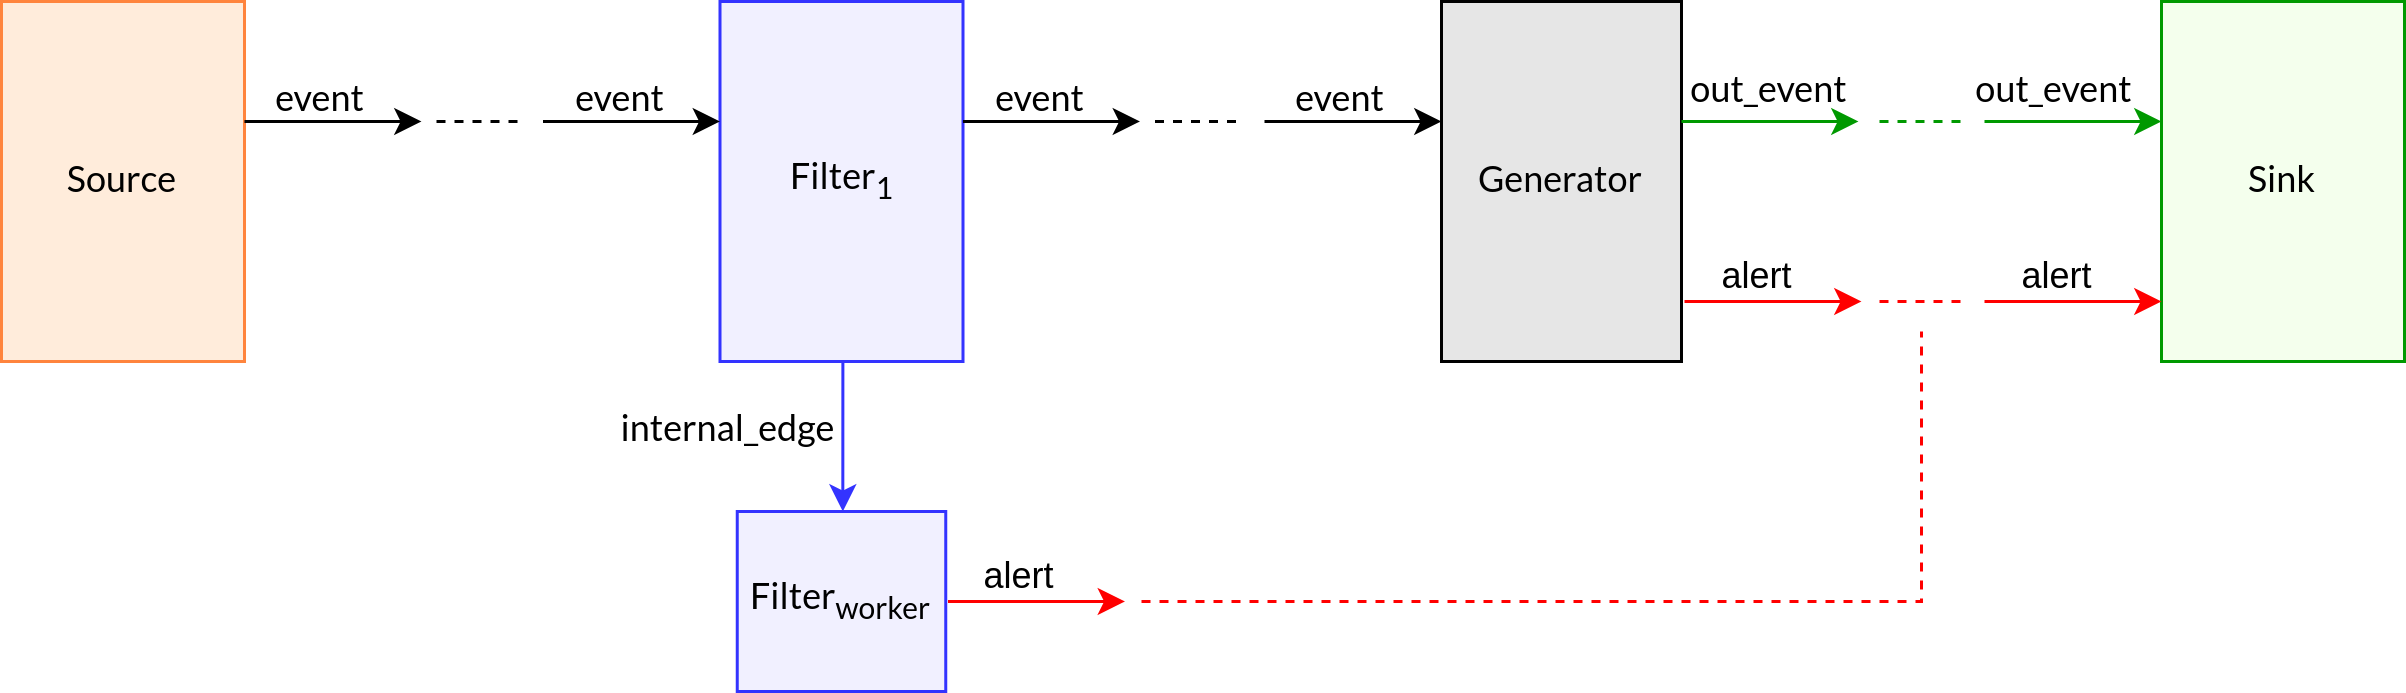
\includegraphics[scale = 0.7]{images/3-Engine/pipeline-schema-filter-detail-old.png}
  \caption{Pipeline Schema with Filter detail}
  \label{img:pipeline-schema-0}
\end{figure}

\begin{figure}[H]
  \centering
  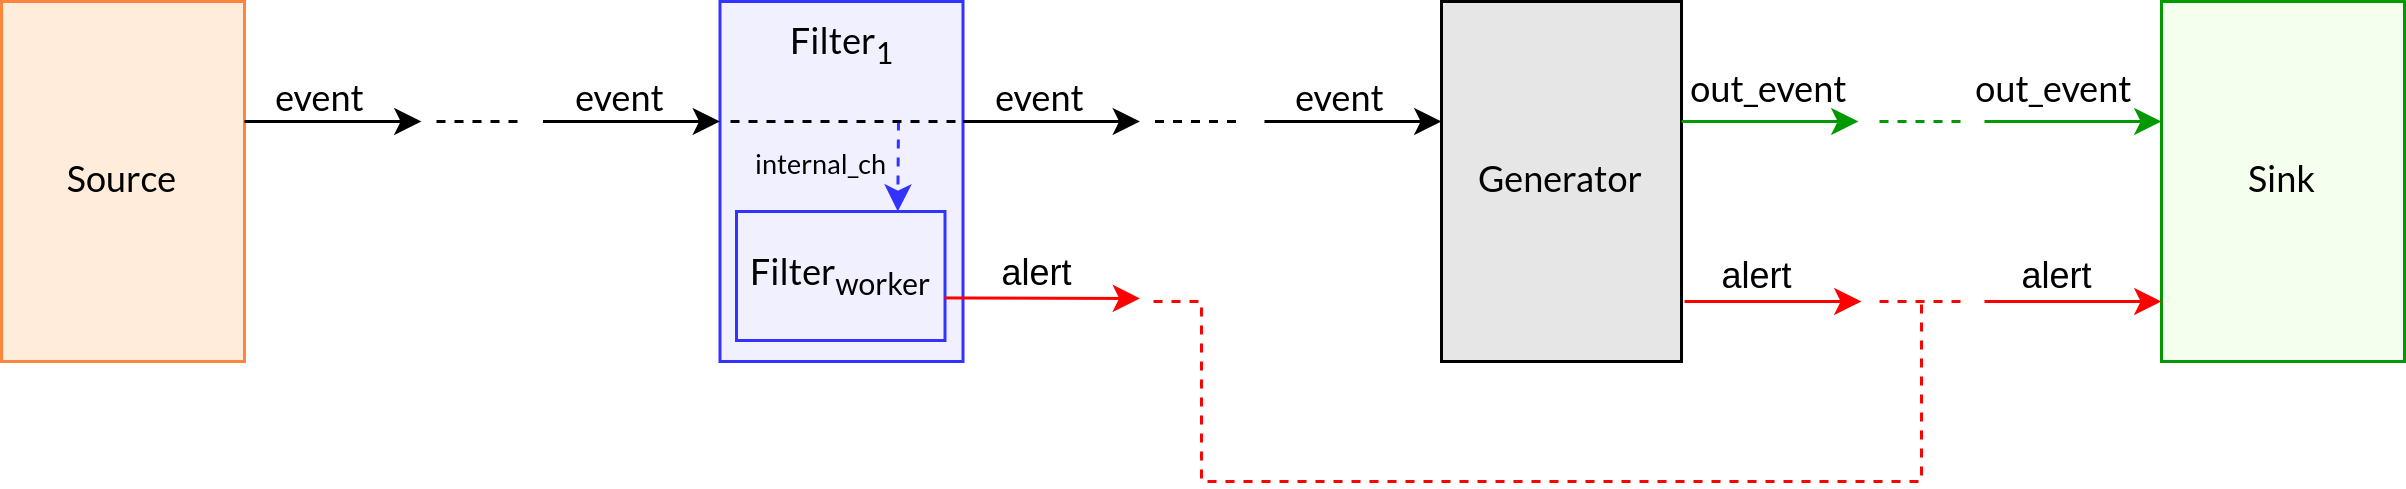
\includegraphics[scale = 0.7]{images/3-Engine/pipeline-schema-filter-detail-1.png}
  \caption{Pipeline Schema with Filter detail 1}
  \label{img:pipeline-schema-1}
\end{figure}

\begin{figure}[H]
  \centering
  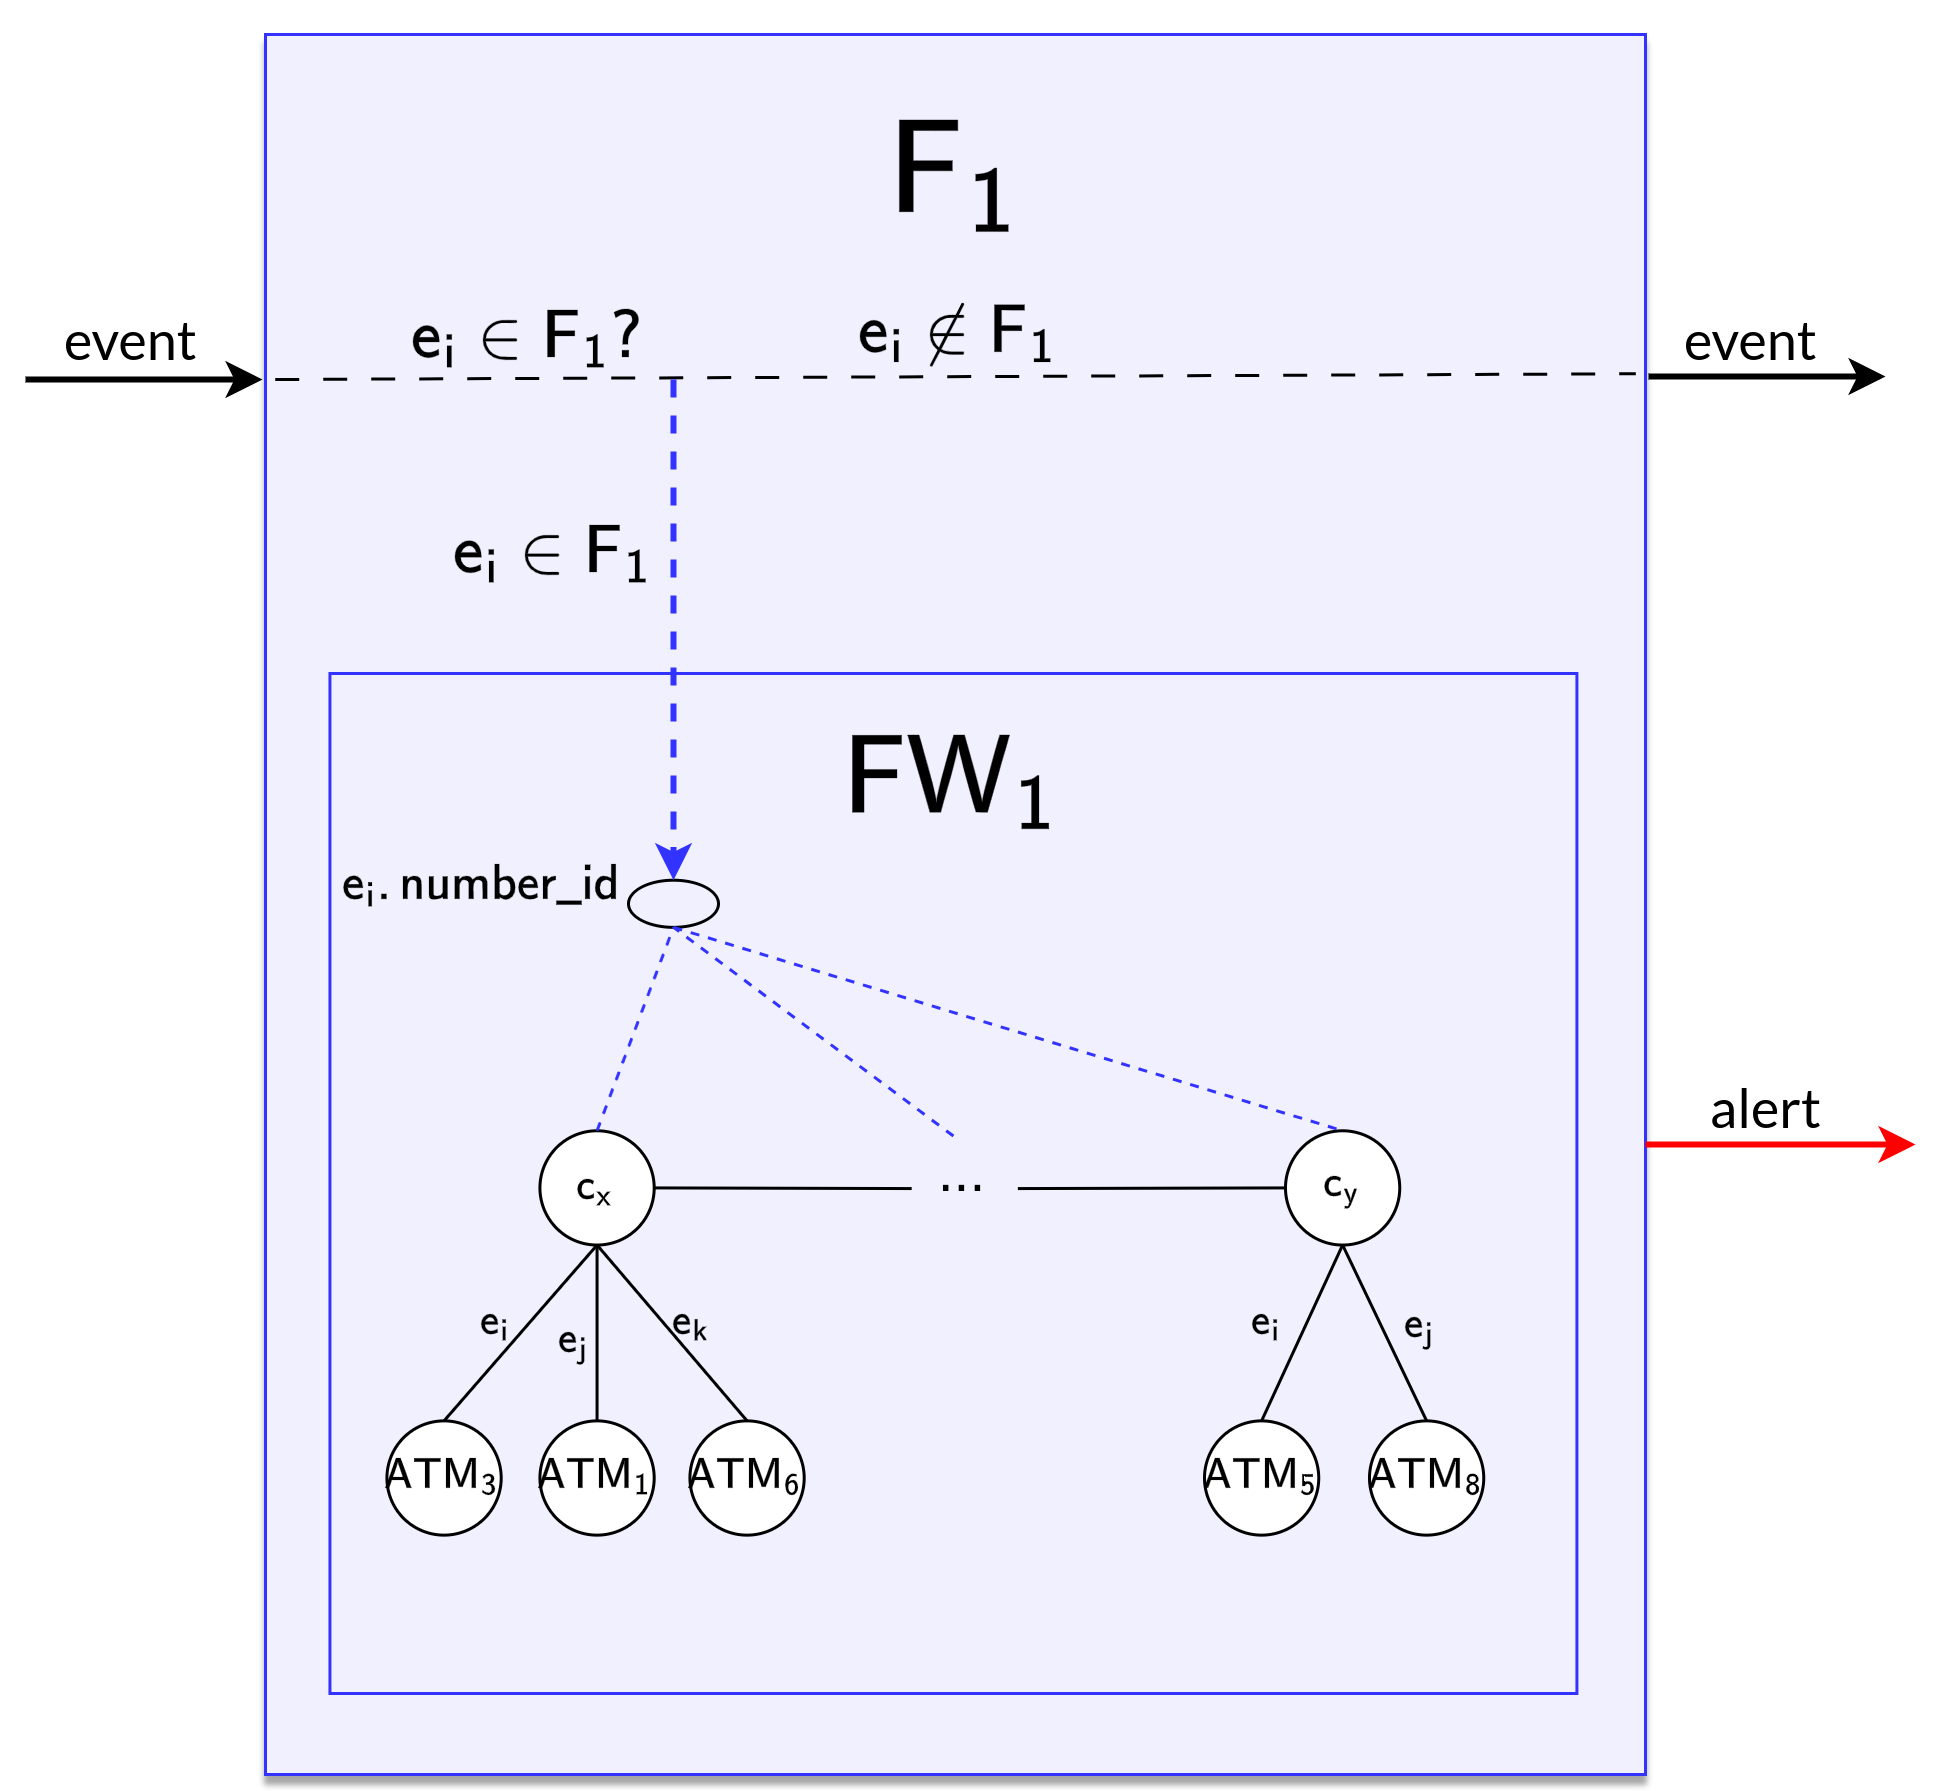
\includegraphics[scale = 0.6]{images/3-Engine/filter-worker-subgraphs.png}
  \caption{\filterworker detail. The subgraphs data structures are shown on it.}
  \label{img:filterworker-subgraphs}
\end{figure}
